\documentclass{standalone}
\usepackage{tikz}
\usepackage{tikz-network}
\usepackage{libertine}
\usepackage{libertinust1math}
\usepackage[T1]{fontenc}
\usetikzlibrary{patterns.meta,decorations.pathmorphing}

\begin{document}
	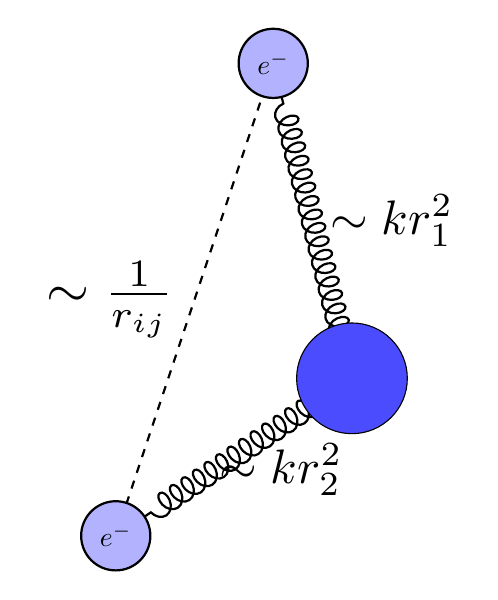
\begin{tikzpicture}
%		\node[anchor=south west,inner sep=0] at (0,0) {\includegraphics[width=\textwidth,]{../../plots/harmonic_potential.png}};
		
		\draw[decorate,decoration={segment length=5pt,aspect=0.7,amplitude=4pt,
			pre=lineto,pre length=5mm,post=lineto,post length=5mm},thick,dashed] (3,4) -- (5, 10) node[midway,left,scale=2] {$\sim \frac{1}{r_{ij}}$};
		
		 \draw[decorate,decoration={coil,segment length=5pt,aspect=0.7,amplitude=4pt,
			pre=lineto,pre length=5mm,post=lineto,post length=5mm},thick] (6,6) -- (3,4)
			node[pos=0.3, below ,scale=1.75, distance=2] {$\sim {kr_2^2}$}
			node[circle, fill=blue!30, draw=black, minimum size=25pt] {$e^{-}$};

		 \draw[decorate,decoration={coil,segment length=5pt,aspect=0.7,amplitude=4pt,
			pre=lineto,pre length=5mm,post=lineto,post length=5mm},thick] (6,6) -- (5,10)
		node[midway,right,scale=1.75] {$\sim {kr_1^2}$}
			node[circle, fill=blue!30, draw=black, minimum size=25pt] {$e^{-}$};
			
		\draw (6,6) node[circle, fill=blue!70, draw=black, minimum size=40pt] {};
		\end{tikzpicture}
\end{document}